\documentclass[11pt]{article}
\usepackage[margin=1in]{geometry}
\usepackage{times}
\usepackage{hyperref}
\usepackage{graphicx}
\usepackage{amsmath, amssymb}
\usepackage{booktabs}
\usepackage{caption}
\usepackage{subcaption}
\usepackage{float}

\graphicspath{{references/plots/}}

\title{Home Credit -- Credit Risk Model Stability\\ Milestone 2}
\author{
\begin{tabular}{cc}
\textbf{Matei-Constantin Goidan} & \textbf{Giulia \c{S}tefania Imbrea} \\
\texttt{matei.goidan@stud.acs.upb.ro} & \texttt{giulia.imbrea@stud.acs.upb.ro}
\end{tabular}
}
\date{May 2026}

\begin{document}

\maketitle

\section{Introduction and Milestone 1 Recap}

The competition is binary loan-default classification scored by a \emph{Gini stability metric} that combines mean weekly Gini, a penalty on a negative time trend, and a penalty on residual variance around that trend. The data spans 92 weeks (\texttt{WEEK\_NUM} 0--91), with 1{,}526{,}659 applicants across 17 tables organised hierarchically (depth 0, 1, 2), totalling approximately 26~GB uncompressed. Class imbalance is 30.8:1 in favour of non-defaulters \cite{kaggle}.

In Milestone~1 we submitted two LightGBM \cite{lightgbm} solutions. \textbf{Submission~1} used the depth-0 join (\texttt{train\_base} + \texttt{train\_static\_0} + \texttt{train\_static\_cb\_0}, 224 features) and scored public 0.4864, private 0.3995 on Kaggle. \textbf{Submission~2} added per-\texttt{case\_id} aggregates from four depth-1 tables and a 10\% stability filter on the coefficient of variation of weekly feature means (673 features), scoring public 0.4879, private 0.3892. Submission~2 improved every validation metric (val AUC 0.8474 vs 0.8188, val Gini-stab 0.6618 vs 0.5975) but \emph{regressed} on the private leaderboard, exposing a gap between our validation horizon (weeks 61--91) and the hidden test horizon ($\approx$ week 100$+$).

\section{Milestone 2 Experiments}

We addressed the four directions proposed at the end of M1: a second model family, model ensembling, walk-forward cross-validation, and metric-aligned hyperparameter optimisation.

\subsection{Submission 3 -- CatBoost on the same feature set}

CatBoost \cite{catboost} was trained on the same 673-feature matrix used by Submission~2. CatBoost handles categorical columns natively (skipping our integer-encoding step) and tends to produce better-calibrated probabilities, relevant since the metric is AUC-based and benefits from well-ordered scores. Categorical columns were passed via \texttt{cat\_features}; the same \texttt{WEEK\_NUM <= 60} time-based split was used.

\textbf{Validation:} AUC 0.8539, Gini-stab 0.6714 -- slightly stronger than Submission~2 locally. \textbf{Kaggle:} public 0.4781, private 0.3903. Useful primarily because the errors are different from LightGBM's, which sets up the ensemble.

\subsection{Submission 4 -- LightGBM + CatBoost 50/50 ensemble}

Naive blend $0.5 \cdot p_{\text{lgb}} + 0.5 \cdot p_{\text{cat}}$ on the test probabilities, using both models with their Submission~2 / Submission~3 settings. Individually LightGBM scored val Gini-stab 0.6618 (AUC 0.8474) and CatBoost 0.6714 (AUC 0.8539); the ensemble achieved val Gini-stab \textbf{0.6703} (AUC 0.8515, residual std 0.0412). On Kaggle: public \textbf{0.4904}, private \textbf{0.4142} -- our best score and the only one exceeding M1's best private score. The mechanism is mechanistic: two model families with similar mean per-week Gini but different error patterns produce, on average, the same mean Gini but with reduced residual variance around the weekly trend -- exactly the term the stability metric penalises.

\subsection{Submission 5 -- Improved LightGBM (walk-forward CV, custom Gini feval, Optuna)}

Three changes layered on top of Submission~2's pipeline, applied only to the LightGBM training procedure (features unchanged):

\textbf{Walk-forward cross-validation.} The single (0--60)/(61--91) split was replaced with three expanding-window folds: (0--40)/(41--60), (0--60)/(61--75), (0--75)/(76--91). This produces a more honest stability estimate than one fold and is necessary for hyperparameter tuning without overfitting to a single validation window.

\textbf{Custom \texttt{feval}.} Instead of optimising AUC (the LightGBM default), early stopping is driven by a custom evaluation function computing the actual Gini-stability score on the validation fold's weekly buckets. The function needs \texttt{WEEK\_NUM} per row, which is not part of LightGBM's \texttt{eval\_metric} signature; we pass it via a module-level variable set before each fold's \texttt{fit} call.

\textbf{Optuna search.} Optuna \cite{optuna} ran a 10-trial search optimising mean walk-forward Gini-stability. Search space: \texttt{learning\_rate} log $[0.01, 0.1]$, \texttt{num\_leaves} $[31, 127]$, \texttt{min\_child\_samples} $[20, 200]$, \texttt{feature\_fraction} $[0.5, 1.0]$, \texttt{bagging\_fraction} $[0.5, 1.0]$, \texttt{reg\_alpha}, \texttt{reg\_lambda} $[0, 1]$.

\textbf{Walk-forward results:} baseline params 0.6401, Optuna-tuned 0.6541 ($+0.014$). Best params: \texttt{learning\_rate}=0.0228, \texttt{num\_leaves}=55, \texttt{min\_child\_samples}=38, \texttt{feature\_fraction}=0.775, \texttt{bagging\_fraction}=0.519, \texttt{reg\_alpha}=0.793, \texttt{reg\_lambda}=0.378. \textbf{Kaggle:} public 0.4859, private 0.3890 -- essentially unchanged from Submission~2 despite the clear local improvement.

\begin{figure}[H]
\centering
\begin{subfigure}[t]{0.48\textwidth}
    \centering
    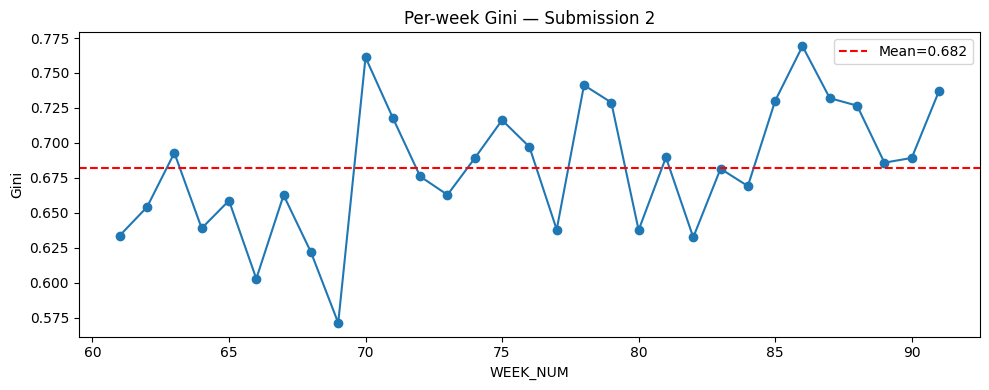
\includegraphics[width=\textwidth]{03_depth1_cell17_plot0.png}
    \caption{Submission~2 (default params).}
\end{subfigure}
\hfill
\begin{subfigure}[t]{0.48\textwidth}
    \centering
    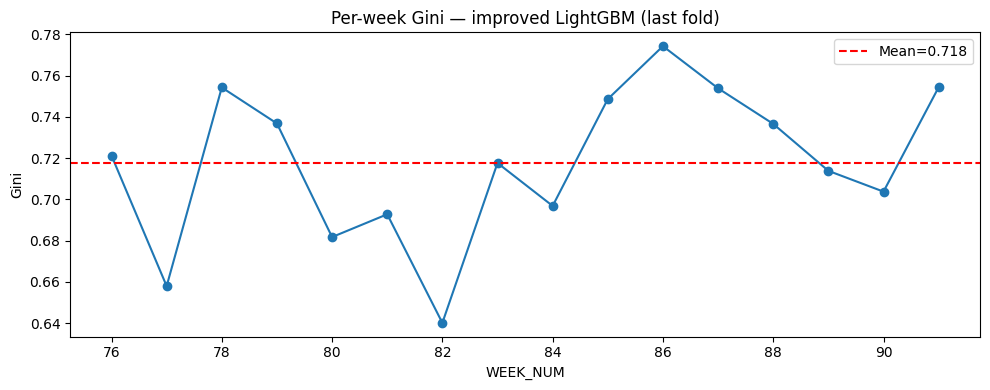
\includegraphics[width=\textwidth]{06_improved_cell19_plot1.png}
    \caption{Submission~5 (Optuna-tuned, last fold).}
\end{subfigure}
\caption{Per-week Gini on the validation fold. Submission~5 raises the mean (0.7157 vs 0.6821 on the matching weeks 76--91) and reduces residual std (0.0299 vs 0.0405), but this does not transfer to the hidden test horizon.}
\label{fig:weekly}
\end{figure}

\subsection{Submission 6 -- Improved ensemble}

Same ensemble structure as Submission~4 but with LightGBM replaced by the Submission~5 version (Optuna-tuned, custom-feval-driven). CatBoost untouched.

\begin{table}[H]
\centering
\caption{Submission 6 validation breakdown (weeks 61--91).}
\label{tab:sub6_val}
\begin{tabular}{lccc}
\toprule
Model & AUC & Gini-stab & Residual std \\
\midrule
LightGBM (Optuna-tuned) alone & 0.8499 & 0.6703 & 0.0390 \\
CatBoost alone                & 0.8489 & 0.6634 & 0.0414 \\
Ensemble 50/50                & \textbf{0.8516} & \textbf{0.6710} & 0.0404 \\
\bottomrule
\end{tabular}
\end{table}

The Optuna-tuned LightGBM individually outperforms Submission~2's LightGBM on local validation (0.6703 vs 0.6618), confirming the tuning did improve in-sample performance. The ensemble barely beats LightGBM alone ($+0.0007$): the two models are now closer in behaviour because the tuned LightGBM uses heavy regularisation that pushes its predictions toward CatBoost-like ones, reducing the diversity that made Submission~4's ensemble effective. \textbf{Kaggle:} public 0.4851, private 0.4029 -- worse than Submission~4 on both. The locally better LightGBM produced a worse ensemble on the hidden test horizon.

\section{Results Summary}

\begin{table}[H]
\centering
\caption{Comparison of all six submissions. Best per column in bold.}
\label{tab:summary}
\begin{tabular}{clcccc}
\toprule
\# & Approach & Val AUC & Val Gini-stab & Kaggle Public & Kaggle Private \\
\midrule
1 & LightGBM, depth-0 only                           & 0.8188 & 0.5975 & 0.4864 & \textbf{0.3995} \\
2 & LightGBM + depth-1 + 10\% stability filter       & 0.8474 & 0.6618 & 0.4879 & 0.3892 \\
3 & CatBoost, same features as Sub.~2                & 0.8539 & 0.6714 & 0.4781 & 0.3903 \\
4 & LightGBM + CatBoost ensemble (50/50)             & 0.8515 & 0.6703 & \textbf{0.4904} & \textbf{0.4142} \\
5 & Sub.~2 LightGBM + walk-forward CV + Optuna       & \textbf{0.8603} & 0.6541$^*$ & 0.4859 & 0.3890 \\
6 & Sub.~5 LightGBM + CatBoost ensemble              & 0.8516 & \textbf{0.6710} & 0.4851 & 0.4029 \\
\bottomrule
\end{tabular}
\caption*{\footnotesize $^*$ Walk-forward CV mean across three folds; the held-out last-fold value is 0.7007.}
\end{table}

\section{Discussion}

\textbf{Ensembling worked, hyperparameter tuning did not transfer.} Submission~4 is our only submission that exceeds M1's best private score (0.4142 vs 0.3995). The ensemble's advantage is mechanistic: averaging two model families with similar mean Gini but different error patterns reduces per-week residual variance directly, which is precisely the term the stability metric penalises. Submission~5's Optuna tuning showed a clear improvement on the walk-forward CV (0.6401 $\rightarrow$ 0.6541) but failed to translate to either Kaggle leaderboard. This repeats the M1 Submission~1 vs Submission~2 pattern at a finer scale: signal that exists in weeks 0--91 does not always exist in the hidden test horizon $\approx$ 100$+$. The Optuna search appears to have overfitted to drift patterns specific to the training weeks, particularly via aggressive regularisation values (\texttt{reg\_alpha}~$=0.79$) that suppressed signal which the default-params LightGBM was using productively.

\textbf{Submission 6 illustrates the same effect for ensembles.} On local validation Submission~6 (0.6710) marginally exceeds Submission~4 (0.6703); on Kaggle it loses 0.011 public and 0.011 private. The tuned LightGBM is closer to CatBoost in behaviour, reducing the diversity that made Submission~4's blend effective. Improvements in either component of an ensemble do not automatically improve the ensemble; what matters is how the components disagree.

\textbf{The hidden test horizon dominates everything.} Across six submissions, every method we tried produced a local validation score that correlates only weakly with Kaggle private. Walk-forward CV gave a better estimate than the single split (and let us tune Optuna at all), but it still uses only weeks $\leq 91$ -- the metric on the private weeks is essentially a different distribution. Methods that helped: ensembling. Methods that hurt or were neutral: more features, hyperparameter tuning, custom evaluation metrics. The conclusion mirrors the competition's own framing -- stability is hardest to estimate from in-sample data.

\begin{figure}[H]
\centering
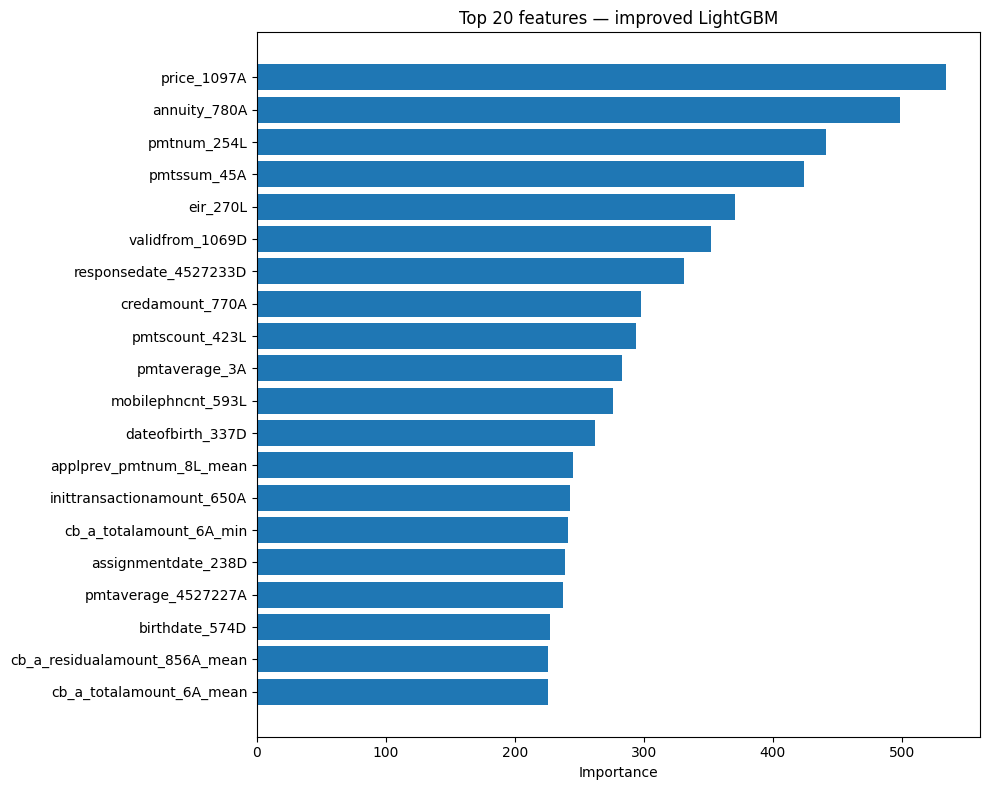
\includegraphics[width=0.7\textwidth]{06_improved_cell21_plot1.png}
\caption{Top 20 feature importances for Submission~5 (LightGBM split count). Depth-0 static fields (\texttt{price\_1097A}, \texttt{annuity\_780A}, \texttt{pmtnum\_254L}) dominate, consistent with Submission~2; the Optuna-tuned params reshuffle their relative ranks but do not surface qualitatively new features.}
\label{fig:importance}
\end{figure}

\textbf{Engineering challenges.} Kaggle's 30~GB notebook RAM was the binding constraint throughout M2. The Submission~2 pipeline alone uses approximately 15~GB at peak (1.5M $\times$ 673 $\times$ float32 $\approx$ 4~GB per matrix, plus LightGBM histogram overhead). Running Optuna on Kaggle exhausted memory after one fold because the search ran on top of an already-loaded feature matrix; we worked around this by running Optuna locally on a 64~GB MacBook Pro M2 Max and hardcoding the best params into the Kaggle notebook. We also encountered Kaggle's hidden-test-set substitution mechanism the hard way: an early ensemble attempt that loaded pre-saved test predictions from an \texttt{.npy} file failed because Kaggle re-runs the notebook with a larger hidden test set at submission time, making pre-computed predictions the wrong length. The fix was to retrain LightGBM during the notebook run with the Optuna-tuned hyperparameters baked in.

\section{Resources, Third-Party Code, and LLM Assistance}

\textbf{Libraries.} Polars (data loading, joining, aggregation under memory pressure), LightGBM \cite{lightgbm}, CatBoost \cite{catboost}, Optuna \cite{optuna}, scikit-learn (\texttt{roc\_auc\_score}), SciPy (\texttt{linregress}), Matplotlib.

\textbf{Kaggle community references.} The competition overview page \cite{kaggle} was used for the exact stability metric formula and weekly bucketing rule. Competition forum discussions on memory management at the 30~GB notebook tier informed our memory strategy. Forum discussions on the hidden test-set substitution at submission time informed our re-architecting of the ensemble notebook after our first failed attempt.

\textbf{LLM assistance.} We used Claude (Anthropic) as a coding assistant throughout M2. Concrete uses: (a) drafting the walk-forward CV loop and the closure pattern for passing \texttt{WEEK\_NUM} into LightGBM's custom \texttt{eval\_metric}; (b) drafting the Optuna \texttt{objective} function and parameter ranges; (c) debugging Polars schema mismatches when concatenating depth-1 parquet shards with mixed null-only columns (the \texttt{diagonal\_relaxed} concat $+$ per-shard cast pattern); (d) writing the patch to the ensemble notebook that loads pre-computed LightGBM test predictions, later reverted in favour of in-notebook retraining once we understood Kaggle's hidden-test-set behaviour. All generated code was read line-by-line, tested locally, and modified before being committed. The assistant was also used for explanatory questions (``what does Kaggle's submission re-run do?'', ``why might Optuna's best params not transfer?'') which directly shaped Section~4. All experimental results, methodology choices, and final interpretations are our own.

\textbf{Code repository.} \url{https://github.com/MateiGoidan/home-credit} (branches: \texttt{main} for the LightGBM-side work in this milestone, \texttt{develop\_catboost} for the CatBoost and ensemble work).

\begin{thebibliography}{9}

\bibitem{kaggle}
Home Credit.
\newblock \emph{Home Credit -- Credit Risk Model Stability.}
\newblock Kaggle Competition. Accessed: 2026-05-20.
\newblock \url{https://www.kaggle.com/competitions/home-credit-credit-risk-model-stability}

\bibitem{lightgbm}
G. Ke, Q. Meng, T. Finley, T. Wang, W. Chen, W. Ma, Q. Ye, T.-Y. Liu.
\newblock LightGBM: A Highly Efficient Gradient Boosting Decision Tree.
\newblock In \emph{Advances in Neural Information Processing Systems (NeurIPS)}, vol.~30, 2017.

\bibitem{catboost}
L. Prokhorenkova, G. Gusev, A. Vorobev, A. Veronika Dorogush, A. Gulin.
\newblock CatBoost: Unbiased Boosting with Categorical Features.
\newblock In \emph{Advances in Neural Information Processing Systems (NeurIPS)}, vol.~31, 2018.

\bibitem{optuna}
T. Akiba, S. Sano, T. Yanase, T. Ohta, M. Koyama.
\newblock Optuna: A Next-generation Hyperparameter Optimization Framework.
\newblock In \emph{Proceedings of the 25th ACM SIGKDD International Conference on Knowledge Discovery \& Data Mining}, 2019.

\bibitem{siddiqi}
N. Siddiqi.
\newblock \emph{Intelligent Credit Scoring: Building and Implementing Better Credit Risk Scorecards.}
\newblock 2nd ed., Wiley, 2017.

\end{thebibliography}

\end{document}
